\documentclass[runningheads]{llncs}
\usepackage[T1]{fontenc}
\usepackage{amsmath,amssymb,booktabs,graphicx}
\usepackage{xcolor}
\usepackage{pgfplots}
\pgfplotsset{compat=1.18}
% Placeholder marker for values that are NOT in the log or the original
% manuscript. Every \tbd must be filled from the analysis output (or the
% sentence removed) before submission. (R2: no \tbd is used.)
\newcommand{\tbd}{\textcolor{red}{\textbf{[TBD]}}}

\begin{document}
\title{Measuring AI-Relatedness in Multilingual Public Procurement Notices: Dictionary-Based Screening, Embedding Classifiers, and Design-Based Inference}
\titlerunning{Measuring AI-Relatedness in Multilingual Procurement Notices}
\author{Jinkyu Lee\orcidID{0000-0002-0886-1572} \and Chang Soo Sung\thanks{Corresponding author.}\orcidID{0000-0001-9284-817X}}
\authorrunning{J. Lee and C. S. Sung}
\institute{Department of Technology Entrepreneurship, Graduate School, Dongguk University, Seoul, Republic of Korea\\ \email{leejinkyu0612@naver.com, redsun44@dgu.ac.kr}}
\maketitle

\begin{abstract}
English keyword lists are a common way to identify AI-related text, but their error in multilingual procurement data and its downstream consequences are seldom quantified. We compared scalable methods for identifying AI-related notices among 54,160 IT and software award notices published in Tenders Electronic Daily (TED) in 2024--2025, of which 6.1\% were in English. A stratified probability sample of 1,199 notices was annotated with a fixed codebook by a primary large language model (LLM) and checked against a second LLM (design-weighted $\kappa=0.77$); no human expert validation was performed. A multilingual dictionary achieved the highest observed F1 (0.63, 95\% CI 0.50--0.78) and doubled the recall of the English dictionary (0.56 vs.\ 0.28). Design-weighted embedding and TF-IDF classifiers performed worse at a fixed 0.5 threshold (F1 0.06 and 0.10); post hoc, either threshold tuning or unweighted training raised the embedding classifier's F1 to 0.34--0.36. The estimated prevalence was 2.32\% with design-based supervised learning (DSL; CI 1.57--3.21\%) and 2.06\% with Horvitz--Thompson estimation (CI 1.38--2.94\%), whereas the English dictionary flagged 0.83\% of notices; the excess persisted under alternative reference labels, but its size depended on four heavily weighted labels. A naive regression suggested that AI-related notices were 4.9 percentage points less likely to report a single tender, but design-based estimates could not determine the sign of any association. Keyword-based AI indicators in procurement need multilingual terms and quantified measurement error before use in inference.\keywords{Public procurement \and AI-relatedness \and Multilingual text classification \and Design-based supervised learning \and Measurement error \and LLM annotation.}
\end{abstract}

%======================================================================
\section{Introduction}
Public procurement is a principal channel through which governments acquire artificial intelligence (AI) systems and services \cite{hickok2022}, and quantifying this market requires deciding which procurement notices concern AI. Text-based measures of AI demand often rely on English keyword lists, as in studies of online vacancies \cite{acemoglu2022,babina2024}, and such lists are a natural choice for procurement notices. They are transparent and cheap, but their accuracy is seldom reported against a reference annotation, and their error is rarely carried into the analyses that use them.

Two features of procurement data make this omission consequential. First, notices in Tenders Electronic Daily (TED) may be published in any of the 24 official EU languages \cite{ahmia2018}; of the 54,160 IT and software award notices analysed here, only 6.1\% were in English, so an English dictionary may miss AI purchases in a language-dependent way. Second, a text-based AI indicator is often used as a regressor in a second-stage analysis, and plugging machine-generated variables into regressions can yield biased estimates and invalid confidence intervals unless the measurement error is addressed \cite{battaglia2025,egami2023}; correction methods also differ in finite samples \cite{audinet2025}.

We therefore examine how the measurement of AI-relatedness affects classification accuracy, the share of AI-related notices, and the association between AI-relatedness and single bidding, a standard indicator of weak competition \cite{fazekas2016}. Six methods---two keyword dictionaries, zero-shot natural language inference (NLI), an embedding-prototype score, and two supervised classifiers---are compared against a codebook-based reference annotation of a stratified probability sample, and design-based supervised learning (DSL) \cite{egami2023} and Horvitz--Thompson (HT) estimation are applied under hypotheses fixed before annotation. No human expert labels were available: the reference labels come from an LLM, checked against a second LLM and selectively re-adjudicated by a third; because such checks do not substitute for expert validation, all influential cases are disclosed. The unit of analysis is the award notice, not the contract or its value.

The study contributes (i) a design-based, language-stratified evaluation of AI-relatedness measurement in multilingual procurement notices; (ii) an assessment of how prevalence estimates depend on the estimator and on a few contested, heavily weighted reference labels; and (iii) an analysis of how measurement uncertainty propagates into competition estimates, with diagnostics that locate when DSL regression becomes uninformative. No new learning algorithm is proposed.

%======================================================================
\section{Related Work}
\subsubsection{Text-based measurement of AI demand.} Labour-economics studies identify AI demand through AI-related terms in job postings \cite{acemoglu2022,babina2024}, and LLMs have been used to score occupational exposure to AI \cite{eloundou2024}. Text-as-data surveys stress that dictionary and supervised measures trade transparency against recall and that their error should be quantified \cite{gentzkow2019}; these studies mainly analyse English text.

\subsubsection{Procurement analytics.} TED data support multilingual corpora \cite{ahmia2018} and national award databases \cite{potin2023}, and single bidding is widely used to assess competition and integrity risk \cite{fazekas2016,decarolis2022}. We are not aware of work that quantifies the error of keyword screening for technology purchases across languages with a probability sample, or that traces this error into competition estimates.

\subsubsection{LLM annotation and inference with predicted variables.} LLMs can match or exceed crowd workers on several annotation tasks \cite{gilardi2023}, but performance varies widely across tasks \cite{ziems2024}, and agreement between LLMs does not establish accuracy because models can share errors. Prediction-powered inference \cite{angelopoulos2023} and DSL \cite{egami2023} combine a small labelled sample with abundant predictions for asymptotically valid estimates, and DSL often, though not uniformly, reduces bias more \cite{audinet2025}. Multilingual encoders \cite{wang2024me5,reimers2020} and NLI-based zero-shot classification \cite{yin2019,he2023} are alternatives to dictionaries whose performance varies by task and language \cite{muennighoff2023}.

%======================================================================
\section{Method}
\subsection{Problem Formulation}
Let $i=1,\dots,N$ index award notices in the analysis frame (one TED publication number each) and let $X_i\in\{0,1\}$ denote AI-relatedness as defined by a fixed codebook. $X_i$ is observed only for a labelled subsample $\mathcal{L}$ drawn with known inclusion probabilities $\pi_i$; for every notice, a method $m$ produces a prediction $\hat{X}^m_i$ or a score. We target (a) the precision, recall, and F1 of each method relative to $X$, (b) the prevalence $\theta=N^{-1}\sum_i X_i$, and (c) the coefficient $\beta$ on $X_i$ in a model of single bidding $Y_i$ with controls $W_i$, defined on the regression subpopulation of Sect.~\ref{sec:data}. The reference annotation defines the construct operationally; it is not treated as expert ground truth.

\subsection{Construct and Reference Annotation}
A notice is AI-related if the procured object includes the development, supply, licensing, operation, or consulting and training on a system whose core functionality relies on AI techniques (machine learning, deep learning, natural language processing or LLMs, chatbots, computer vision, speech recognition or synthesis, or predictive models learned from data). Generic software, workflow automation without AI, dashboards without learning components, and hardware are coded as not AI-related. This definition follows the task-based view of AI in vacancy studies \cite{acemoglu2022} and the procurement-risk framing of AI systems \cite{hickok2022}. Each sampled notice was annotated by a primary LLM (Claude Haiku 5.5) and a secondary LLM (Gemini 2.5 Flash-Lite) with the same zero-shot prompt (temperature 0, JSON output). The pre-specified reference is the primary label $X$; unparsable responses are treated as missing, never as negative. Two pre-specified variants require agreement of both annotators ($X_\wedge$) or either annotator ($X_\vee$); for the 33 notices without a secondary label both variants use the primary label, so they are an intersection and a union only where both labels exist. Post hoc, a third LLM (DeepSeek-Chat-v3.1) re-annotated a selected subset of 123 notices with the same prompt: those whose first two labels disagreed or lacked a secondary label, plus all primary positives in strata C and D. The resulting \emph{selectively adjudicated reference} $X_{\mathrm{adj}}$ takes the majority of the available labels (if only two were available and they differed, the third label decided); all other notices keep the primary label. These procedures assess label sensitivity but do not substitute for independent expert validation; all influential cases are therefore disclosed (Table~\ref{tab:cases}).

\subsection{Measurement Methods}
\textbf{M1} is an English AI dictionary (22 patterns, e.g., \textit{artificial intelligence}, \textit{machine learning}, \textit{chatbot}, \textit{LLM}). \textbf{M2} adds core equivalents of \textit{artificial intelligence}, \textit{machine learning}, \textit{neural network}, \textit{language model}, and \textit{chatbot} in the EU languages and the abbreviations KI and IA. Because M1 and M2 define the sampling strata, both were fixed before sampling and annotation; since M2 also changes the term set, their comparison reflects multilingual coverage and term choice jointly, not a pure language effect. \textbf{M3} is zero-shot NLI with mDeBERTa-v3-base-mnli-xnli \cite{he2023,yin2019} and the hypothesis ``This procurement is about artificial intelligence'' (entailment probability $\ge 0.5$); it is label-free. \textbf{M4} is the maximum cosine similarity between a notice and five English prototype queries in the multilingual-e5-small space \cite{wang2024me5}; the score is label-free, but its threshold is selected within training folds, and its English prototypes make it not language-neutral. \textbf{M5}, the pre-specified embedding-based classifier, is an $L_2$-regularised logistic regression on multilingual-e5-small embeddings trained on the reference labels with weights $1/\pi_i$ and a fixed threshold of 0.5. \textbf{M6} replaces the embeddings with character 3--5-gram TF-IDF features, a strong classical baseline for short multilingual text. All label-trained components, including thresholds and TF-IDF vocabularies, are cross-fitted: predictions for labelled notices come from five folds that exclude them; unlabelled notices are scored by a model refitted on all labels. E5 inputs use the `passage:'/`query:' prefixes with mean pooling.

\subsection{Sampling Design and Design-Based Estimation}
Because AI notices are rare, the frame was stratified: A (M1 hit), B (M2 hit but not M1), C (neither, but M4 similarity in the top 3\%), and D (remaining notices), and simple random samples were drawn without replacement within strata (seed 2027). Inclusion probabilities are $\pi_h=n_h/N_h$, where $n_h$ counts \emph{labelled} notices; in stratum C one of the 250 drawn notices received no parsable primary label, so $\pi_C$ is nonresponse-adjusted and valid if the failure is unrelated to $X$ within the stratum (Table~\ref{tab:design}). Accuracy metrics weight labelled notices by $1/\pi_i$. For prevalence and regression, DSL replaces the unobserved $X_i$ with the pseudo-outcome
\begin{equation}
\tilde{X}_i=\hat{g}(T_i)+\frac{R_i}{\pi_i}\bigl(X_i-\hat{g}(T_i)\bigr),
\label{eq:pseudo}
\end{equation}
where $\hat{g}$ is the cross-fitted M5 probability, $T_i$ the text, and $R_i$ the labelling indicator. For a fixed $\hat{g}$, $E_p(R_i)=\pi_i$ gives $E_p(\tilde{X}_i)=X_i$ under the sampling design, so $\hat\theta_{\mathrm{DSL}}=N^{-1}\sum_i\tilde{X}_i$ is design-unbiased (given the nonresponse assumption) whatever the accuracy of $\hat{g}$, which affects only its variance. Under appropriate sampling and cross-fitting regularity conditions, DSL permits asymptotically valid inference without requiring a correctly specified auxiliary predictor \cite{egami2023}. Our implementation meets these conditions only approximately, because unlabelled notices are scored by a predictor trained on all labels; we claim neither finite-sample unbiasedness nor exact asymptotic validity, and our intervals, which hold $\hat{g}$ fixed, omit the uncertainty of estimating it. Setting $\hat{g}\equiv0$ yields the HT estimator. If $\hat{g}$ is constant within strata, as the M1 and M2 indicators are, $\hat\theta_{\mathrm{DSL}}$ reduces algebraically to $\hat\theta_{\mathrm{HT}}$; a predictor can therefore improve on HT only through within-stratum variation, chiefly in stratum D.

For the linear probability model $Y_i=\beta X_i+W_i^\top\gamma+\varepsilon_i$ on the regression sample $\mathcal{R}$ ($N_R$ notices), every OLS moment is linear in $X_i$ because $X_i^2=X_i$, so $\tilde{X}_i$ replaces $X_i$ wherever it appears:
\begin{equation}
\hat{A}=\frac{1}{N_R}\sum_{i\in\mathcal{R}}\begin{pmatrix}\tilde{X}_i & \tilde{X}_iW_i^\top\\ W_i\tilde{X}_i & W_iW_i^\top\end{pmatrix},\quad
\hat{b}=\frac{1}{N_R}\sum_{i\in\mathcal{R}}\begin{pmatrix}\tilde{X}_iY_i\\ W_iY_i\end{pmatrix},\quad
(\hat\beta,\hat\gamma^\top)^\top=\hat{A}^{-1}\hat{b}.
\label{eq:moments}
\end{equation}
The upper-left entry uses $\tilde{X}_i$, not $\tilde{X}_i^2$. Because $\tilde{X}_i$ can be negative or far above one, $\hat{A}$ need not be positive definite; we report its condition number, $\mathrm{cond}(\hat{A})$. Labelled notices in $\mathcal{R}$ keep their frame inclusion probabilities. Prevalence CIs are stratified bootstrap intervals; for regression we report sandwich standard errors and, for the pre-specified DSL estimate, a bootstrap interval. A linear probability model is used because the specification contains over 100 fixed effects, for which logit estimates are less stable.

%======================================================================
\section{Experimental Setup}
\subsection{Data}
\label{sec:data}
We retrieved all TED contract award notices (eForms type \texttt{can-standard}) published between 1 January 2024 and 31 December 2025 whose CPV classification falls under IT services (72000000) or software packages (48000000), using the public TED Search API v3 (reuse permitted under the European Commission's reuse policy). After deduplication by publication number (CPV matching includes additional CPV codes), 55,508 notices from 50 buyer countries in 23 languages remained; excluding notices with fewer than ten characters of title and description left an analysis frame of $N=54{,}160$, of which 3,308 (6.1\%) were in English. The text of a notice is its procedure title and description in its first official language (median 378 characters, truncated at 2,000). No personal data are used, and notice texts are not redistributed.

Of the 54,160 frame notices, 17,864 report no received-tenders count, 4,635 report more than one (lot-level counts in multi-lot notices), and 31,661 report exactly one. Because eForms records this count per lot result, a notice with one reported count need not concern a single lot. Excluding counts of zero (1,271; no tender, outside the single-bidding estimand) and above 100 (2; probable recording errors, cf.\ \cite{potin2023}) left a regression sample $\mathcal{R}$ of 30,388 notices (630 labelled). The outcome $Y_i$ indicates that the notice's single reported count of tenders (eForms received-submissions type `tenders', not the SME or electronic sub-counts) equals one; it is a notice-level proxy, and 46.2\% of $\mathcal{R}$ had $Y_i=1$. The regression estimand therefore pertains to notices with eligible reported tender counts rather than to the entire frame. Design weights do not correct for selection into $\mathcal{R}$; post hoc, $\mathcal{R}$ contained fewer English notices than the 23,772 excluded notices (3.9\% vs.\ 9.0\%) but had similar flag rates (M1 0.82\% vs.\ 0.85\%; M2 1.55\% vs.\ 1.72\%). Controls are fixed effects for buyer country (absorbing institutional differences and the currency of the contract value), CPV division (26 levels after pooling divisions with fewer than 30 notices), procedure type, buyer legal type, and publication quarter, plus log contract value with a missing-value indicator \cite{fazekas2016,decarolis2022}.

\subsection{Sample, Annotation, and Implementation}
Table~\ref{tab:design} reports the sampling design. The 1,200 sampled notices were annotated by both LLMs through OpenRouter between 11:54 and 12:16 KST on 27 November 2026 (2,400 requests; US\$0.14). Of the 1,199 labelled notices, 364 were coded AI-related (an unweighted count; frame estimates use the weights). The secondary model returned unparsable text for 86 notices; re-querying them with the same prompt and a 120-token output limit recovered 53, leaving 33 without a secondary label (17 in stratum D, 11 in B, 3 in A, 2 in C). The re-query and the adjudication (275 requests) cost US\$0.03. On eight CPU threads, the dictionaries processed the frame in 7--20\,s, e5 embedding took 1,229\,s, and NLI about 4\,s per notice. Bootstrap CIs use 2,000 resamples drawn with replacement within strata of the labelled sample; classifiers and thresholds are not refitted within replicates, so these CIs reflect label sampling only. Resampling with replacement ignores the finite-population correction, which is conservative for strata A and B and immaterial for prevalence, whose uncertainty is driven almost entirely by stratum D (sampling fraction below 0.01).

\begin{table}[t]
\caption{Stratified reference sample. $N_h$: frame notices; drawn: sampled notices; $n_h$: notices with a parsable primary label; $\pi_h=n_h/N_h$ (for D, $450/51{,}756$); Pos.: notices coded AI-related by the primary annotator; Est.: weighted estimate of AI-related notices in the stratum.}\label{tab:design}
\centering
\begin{tabular}{llrrrrrr}
\toprule
Stratum & Definition & $N_h$ & Drawn & $n_h$ & $\pi_h$ & Pos. & Est. \\
\midrule
A & English-dictionary hit (M1) & 450 & 250 & 250 & 0.556 & 172 & 310 \\
B & Multilingual-dictionary hit only (M2) & 428 & 250 & 250 & 0.584 & 183 & 313 \\
C & No hit; M4 score in top 3\% & 1,526 & 250 & 249 & 0.163 & 5 & 31 \\
D & Remaining notices & 51,756 & 450 & 450 & 0.009 & 4 & 460 \\
\midrule
Total & & 54,160 & 1,200 & 1,199 & & 364 & 1,114 \\
\bottomrule
\end{tabular}
\end{table}

\subsection{Pre-specified Hypotheses and Testing}
The analysis plan was fixed before annotation and committed to the project repository (commit 7314e8d, 27 November 2026, 11:12 KST; amendment commit b1eb797, 12:22 KST), a time-stamped commit rather than an external registration. It stated: \textbf{H1} the recall of M1 is lower for non-English than for English notices, i.e., $\Delta_{\mathrm{H1}}=R_{\mathrm{non}}-R_{\mathrm{EN}}<0$; \textbf{H2} M5 attains higher F1 than M1 (H2a) and M2 (H2b); \textbf{H3} the DSL prevalence exceeds the M1 prevalence; and \textbf{H4} the DSL coefficient on AI-relatedness in the single-bidding model differs from zero (two-sided). One-sided bootstrap $p$-values for the four tests H1, H2a, H2b, and H3 are Holm-adjusted as one family; H4 is assessed by its 95\% CI. All reported CIs are unadjusted 95\% intervals. One amendment, recorded before the affected results were computed, restricted M3 to the labelled sample because its projected CPU time for the frame exceeded the plan's six-hour rule; M3 is therefore evaluated for accuracy only. Analyses added after inspecting results, including the adjudication, the re-query, and all HT comparisons, exact intervals, ablations, diagnostics, and leave-one-out (LOO) analyses, are labelled post hoc and support no confirmatory claim.

%======================================================================
\section{Results}
\subsection{Reference Annotation}
Among the 1,166 notices with both labels after the re-query, unweighted $\kappa$ was 0.92 and design-weighted $\kappa$ 0.77 (95\% CI 0.60--0.95); weighted positive and negative specific agreement were 0.78 and 0.996. Weighted $\kappa$ was lower for English (0.48) than for non-English notices (0.82); the unweighted--weighted gap reflects disagreement in the heavily weighted unflagged strata. Table~\ref{tab:cases} lists all nine primary positives in strata C and D. Each stratum-D notice carries a weight of about 115, so the four stratum-D positives account for 460 of the 1,114 estimated AI-related notices (41\%). The secondary model coded one of them AI-related (biometric face detection) and the third model also the train-running forecast module, so $X_{\mathrm{adj}}$ retains two of the four stratum-D and four of the five stratum-C positives (359 positives in total).

\begin{table}[t]
\caption{All primary-reference positives in the unflagged strata C and D, with the labels of the secondary (S) and third (T) LLM and the selectively adjudicated reference $X_{\mathrm{adj}}$. Objects are paraphrased from the notice text. Post hoc.}\label{tab:cases}
\centering
\begin{tabular}{llllccc}
\toprule
Notice & Str. & Lang. & Procured object (paraphrased) & S & T & $X_{\mathrm{adj}}$ \\
\midrule
192940-2025 & C & ENG & Digital dictation and voice-recognition system & 1 & 1 & 1 \\
86787-2024  & C & ENG & Biometric authentication with facial recognition & 1 & 1 & 1 \\
327445-2025 & C & ENG & Operation and development of a statistical model & 0 & 0 & 0 \\
678350-2025 & C & SPA & Voice assistant for primary-care appointments & 1 & 1 & 1 \\
810556-2025 & C & ENG & Reseller services for Darktrace software & 1 & 1 & 1 \\
755854-2025 & D & SPA & Access to specialised genetics software & 0 & 0 & 0 \\
787623-2025 & D & RON & Integrated e-services platform and licences & 0 & 0 & 0 \\
500255-2024 & D & ENG & Train-running forecast information (TIS) & 0 & 1 & 1 \\
201930-2025 & D & CES & Support of a biometric face-detection system & 1 & 1 & 1 \\
\bottomrule
\end{tabular}
\end{table}

\subsection{Classification Accuracy (H1, H2)}
Table~\ref{tab:acc} reports design-weighted accuracy. M2 achieved the highest observed F1 (0.63, 95\% CI 0.50--0.78), doubling the recall of M1 (0.56 vs.\ 0.28) at similar observed precision (0.71 vs.\ 0.69); no test of M2 against the other methods was pre-specified. H1 was not supported under the primary reference: the recall of M1 was 0.25 for English and 0.28 for non-English notices ($\Delta_{\mathrm{H1}}=0.04$ from unrounded recalls, CI $-0.55$ to 0.27), largely because one English stratum-D positive carries a large weight. M3 was precise (0.96) but missed most AI-related notices (recall 0.11). H2 was not supported, and the observed differences had the opposite sign: at the 0.5 threshold, M5 and M6 predicted almost no positives (recall 0.03 and 0.05; F1 0.06 and 0.10), although M5 had the highest AUPRC among pre-specified methods (0.33). The F1 differences M5$-$M1 ($-0.34$, CI $-0.45$ to $-0.26$) and M5$-$M2 ($-0.57$, CI $-0.70$ to $-0.45$) were negative (Holm-adjusted $p=1.00$ for both). A post hoc $2\times2$ ablation separated training weights from thresholding: M5's F1 was 0.06 with weights at 0.5, 0.34 with weights and a fold-tuned threshold, 0.36 without weights at 0.5, and 0.35 without weights and with a tuned threshold (M5u). Either change alone raised F1 to a similar level, so the failure arose from combining design-weighted training with a fixed 0.5 threshold; M5u remained below M2 (difference $-0.28$, CI $-0.39$ to $-0.18$). M2 remained the best method under $X_{\mathrm{adj}}$, $X_\wedge$, and $X_\vee$ (F1 0.66, 0.73, 0.64), with a paraphrase-multilingual-MiniLM encoder (M5 F1 0.30), and for non-English notices (F1 0.40, 0.66, 0.05 for M1, M2, M5). $\Delta_{\mathrm{H1}}$ was 0.06 (CI $-0.61$ to 0.29) under $X_{\mathrm{adj}}$ and $-0.32$ (CI $-0.61$ to $-0.06$) under $X_\wedge$.

\begin{table}[t]
\caption{Design-weighted accuracy against the primary reference ($n=1{,}199$). R$_\mathrm{EN}$/R$_\mathrm{non}$: recall for English/non-English notices. AUPRC only for score-based methods. $^\S$Labelled sample only (amendment); excluded from prevalence and regression. $^\dagger$Post hoc variant (unweighted training, fold-internal threshold), not part of the pre-specified tests.}\label{tab:acc}
\centering
\begin{tabular}{lrrrrrr}
\toprule
Method & Precision & Recall & R$_\mathrm{EN}$ & R$_\mathrm{non}$ & F1 [95\% CI] & AUPRC \\
\midrule
M1 English dictionary & 0.69 & 0.28 & 0.25 & 0.28 & 0.40 [0.30, 0.53] & -- \\
M2 Multilingual dictionary & 0.71 & 0.56 & 0.26 & 0.62 & 0.63 [0.50, 0.78] & -- \\
M3 Zero-shot NLI$^\S$ & 0.96 & 0.11 & 0.04 & 0.13 & 0.20 [0.14, 0.31] & 0.27 \\
M4 Prototype similarity & 0.08 & 0.31 & 0.94 & 0.18 & 0.13 [0.08, 0.23] & 0.07 \\
M5 Embedding + LR & 1.00 & 0.03 & 0.05 & 0.03 & 0.06 [0.03, 0.11] & 0.33 \\
M6 TF-IDF + LR & 0.97 & 0.05 & 0.03 & 0.05 & 0.10 [0.06, 0.16] & 0.27 \\
M5u$^\dagger$ Embedding + LR & 0.41 & 0.30 & 0.08 & 0.35 & 0.35 [0.25, 0.50] & 0.34 \\
\bottomrule
\end{tabular}
\end{table}

\subsection{Prevalence (H3)}
The HT estimate of the share of AI-related notices was 2.06\% (SE 0.42 points; CI 1.38--2.94\%) and the DSL estimate with M5 2.32\% (SE 0.42; CI 1.57--3.21\%) (Fig.~\ref{fig:prev}); DSL thus did not improve precision over HT. Frame flag rates were 0.83\% (M1), 1.62\% (M2), 6.51\% (M4), and below 0.2\% (M5, M6). The DSL estimate exceeded the M1 share by 1.49 points (CI 0.73--2.38; Holm-adjusted $p=0.002$), supporting H3: the English dictionary flagged notices at approximately one third of the DSL-estimated prevalence. As M1 also flags false positives, this ratio is not its detection rate (recall 0.28). Post hoc, the HT estimate exceeded the M1 share by 1.23 points (CI 0.55--2.11), so the finding is not specific to the auxiliary predictor. Its direction does not hinge on stratum D, since the point estimates for strata A--C in Table~\ref{tab:design} already exceed the 450 notices flagged by M1 (stratum A); its magnitude does. The stratum-D rate of 4/450 has an exact (Clopper--Pearson) 95\% interval of 0.0024--0.0226, implying 126--1,170 AI-related notices in the stratum (point estimate 460) and a contribution of 0.23--2.16 points to the frame share. The excess persisted under every alternative reference, with differences from the M1 share of 1.01 ($X_{\mathrm{adj}}$; CI 0.38--1.83), 0.57 ($X_\wedge$; CI 0.26--1.08), and 1.52 points ($X_\vee$; CI 0.78--2.43). Omitting one stratum-D positive lowered the DSL prevalence to 2.11\%, omitting one stratum-C positive to 2.31\%. The unparsed stratum-C notice could shift the stratum-C estimate by at most about one stratum-C weight (about six notices), comparable to that omission; coding it alternatively as zero and one was not computed.

\begin{figure}[t]
\centering
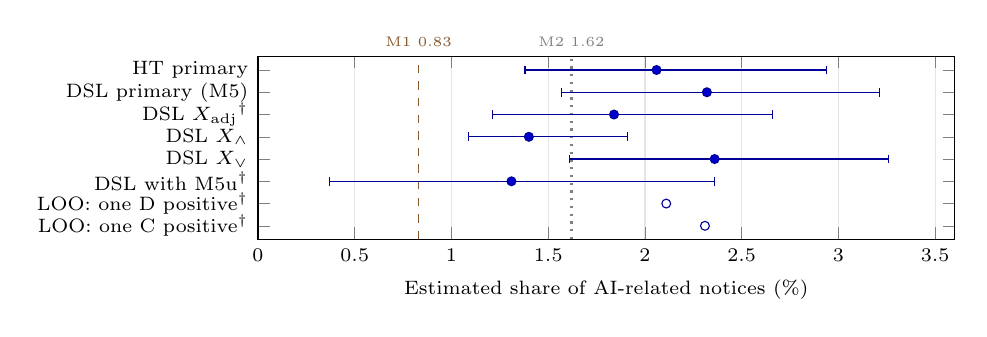
\begin{tikzpicture}
\begin{axis}[width=0.86\linewidth,height=3.9cm,xmin=0,xmax=3.6,ymin=0.4,ymax=8.6,
  ytick={1,...,8},
  yticklabels={LOO: one C positive$^\dagger$,LOO: one D positive$^\dagger$,DSL with M5u$^\dagger$,DSL $X_\vee$,DSL $X_\wedge$,DSL $X_{\mathrm{adj}}$$^\dagger$,DSL primary (M5),HT primary},
  tick label style={font=\scriptsize},label style={font=\scriptsize},
  xlabel={Estimated share of AI-related notices (\%)},xtick={0,0.5,...,3.5},
  xmajorgrids,major grid style={gray!20},clip=false]
\draw[dashed,brown!70!black] (axis cs:0.83,0.4) -- (axis cs:0.83,8.6) node[above,font=\tiny]{M1 0.83};
\draw[dotted,thick,gray] (axis cs:1.62,0.4) -- (axis cs:1.62,8.6) node[above,font=\tiny]{M2 1.62};
\addplot+[only marks,mark=*,mark size=1.6pt,color=blue!60!black,
  error bars/.cd,x dir=both,x explicit]
  coordinates {(2.06,8) += (0.88,0) -= (0.68,0)
               (2.32,7) += (0.89,0) -= (0.75,0)
               (1.84,6) += (0.82,0) -= (0.63,0)
               (1.40,5) += (0.51,0) -= (0.31,0)
               (2.36,4) += (0.90,0) -= (0.75,0)
               (1.31,3) += (1.05,0) -= (0.94,0)};
\addplot+[only marks,mark=o,mark size=1.6pt,color=blue!60!black] coordinates {(2.11,2) (2.31,1)};
\end{axis}
\end{tikzpicture}
\caption{Design-based prevalence estimates with 95\% stratified bootstrap CIs (open circles: point estimates only). Vertical lines: frame flag rates of M1 and M2, which have no sampling error. $^\dagger$Post hoc.}\label{fig:prev}
\end{figure}

\subsection{AI-Relatedness and Single Bidding (H4)}
\label{sec:reg}
With naive plug-in indicators (Table~\ref{tab:reg}), M2 suggested that AI-related notices were 4.9 points less likely to report a single tender (CI $-8.9$ to $-0.8$), whereas M1 ($-1.7$, CI $-7.3$ to 3.9) and the other methods gave CIs that included zero; a logit plug-in model reproduced this sign pattern (M2 odds ratio 0.77, SE of log-odds 0.11). The labelled-only estimate was 3.1 points (CI $-8.0$ to 14.1; $n=630$). The pre-specified DSL estimate was uninformative ($\hat\beta=-124.2$ points, sandwich SE 1,812; bootstrap CI $-495$ to 429; the gap between the intervals itself signals instability). H4 was therefore not supported; the estimates were inconclusive about the sign and size of the association.

Post hoc diagnostics (Fig.~\ref{fig:diag}) locate the instability. The pseudo-outcomes reach 113.6 with M5 and 115.0 with the M2 indicator, values produced by stratum-D positives with near-zero predictions. Without controls DSL with M5 or the M2 indicator was stable (SE 9.3 and 9.7 points), and country fixed effects raised $\mathrm{cond}(\hat{A})$ to $1.69\times10^4$ with little change in SE; the remaining controls raised it to about $3\times10^6$ and the SE to 467--1,799 points. M5u did not follow this pattern, so $\mathrm{cond}(\hat{A})$, nearly equal across predictors for a given control set, does not by itself explain the instability; an interaction between a few extreme pseudo-outcomes and the fixed-effect design is plausible but was not decomposed. Open procedures contain no heavily weighted stratum-D positive (maximum pseudo-outcome 6.1), and there DSL with full controls was stable (1.0 points, SE 6.3); the naive estimates were $-2.0$ (M1; CI $-9.0$ to 5.0) and $-4.8$ points (M2; CI $-9.9$ to 0.3), and the labelled-only estimate 2.0 (CI $-9.6$ to 13.7; $n=430$). The restriction also bears on construct validity, because single-bid shares in $\mathcal{R}$ ranged from 38.6\% in open procedures to 93.9\% in negotiated procedures without prior call ($n=4{,}379$), where one tender is often inherent; as the no-control estimates ignore this composition, they are not read as associations. Precision also rose as fewer stratum-D positives remained in the reference ($X_{\mathrm{adj}}$, $X_\wedge$; Table~\ref{tab:reg}). In a synthetic check (true coefficient 0.10, deliberately miscalibrated predictor, 200 replications), the estimator was close to the truth on average (mean 0.115, median 0.153) relative to its dispersion (mean SE 2.27), but 95\% sandwich intervals covered it in only 86\% of replications, which argues against a coding error but shows under-coverage.

\begin{table}[t]
\caption{Coefficient on AI-relatedness in a linear probability model of single bidding ($n=30{,}388$ notices with an eligible reported tender count; fixed effects for country, CPV division, procedure, buyer type, and quarter; log value). Percentage points with 95\% sandwich CIs unless noted. $^\dagger$Post hoc. $^\ddagger$Stratified bootstrap CI; sandwich SE 1,812.}\label{tab:reg}
\centering
\begin{tabular}{lrrr}
\toprule
Measurement of AI-relatedness & AI notices & $\hat\beta$ & 95\% CI or (SE) \\
\midrule
M1 English dictionary (naive) & 249 & $-1.7$ & [$-7.3$, 3.9] \\
M2 Multilingual dictionary (naive) & 470 & $-4.9$ & [$-8.9$, $-0.8$] \\
M4 Prototype similarity (naive) & 1,575 & $-1.2$ & [$-3.6$, 1.3] \\
M5 Embedding + LR (naive) & 31 & 2.7 & [$-12.2$, 17.6] \\
M6 TF-IDF + LR (naive) & 34 & $-11.4$ & [$-24.2$, 1.3] \\
Labelled notices only (weighted) & -- & 3.1 & [$-8.0$, 14.1] \\
DSL with M5 (pre-specified) & -- & $-124.2$ & [$-495$, 429]$^\ddagger$ \\
DSL with M5, $X_{\mathrm{adj}}$ reference$^\dagger$ & -- & $-42.2$ & (177.2) \\
DSL with M5, $X_\wedge$ reference & -- & 6.0 & [$-6.7$, 18.8] \\
DSL with M5u$^\dagger$ & -- & $-24.9$ & [$-103.1$, 53.4] \\
\bottomrule
\end{tabular}
\end{table}

\begin{figure}[t]
\centering
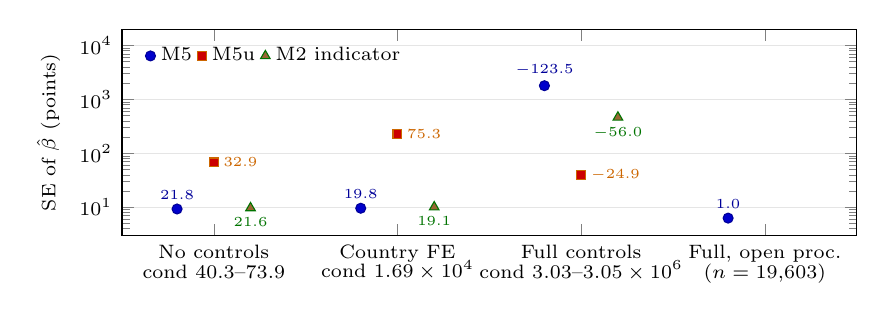
\begin{tikzpicture}
\begin{axis}[width=0.9\linewidth,height=4.2cm,ymode=log,ymin=3,ymax=2e4,
  xmin=0.5,xmax=4.5,xtick={1,2,3,4},
  xticklabels={{No controls\\[-1pt]cond 40.3--73.9},{Country FE\\[-1pt]cond $1.69\times10^4$},{Full controls\\[-1pt]cond $3.03$--$3.05\times10^6$},{Full, open proc.\\[-1pt]($n=19{,}603$)}},
  xticklabel style={align=center,font=\scriptsize},yticklabel style={font=\scriptsize},
  ylabel={SE of $\hat\beta$ (points)},label style={font=\scriptsize},
  ymajorgrids,major grid style={gray!20},
  legend style={font=\scriptsize,at={(0.02,0.97)},anchor=north west,draw=none,fill=none},legend columns=3,
  nodes near coords,point meta=explicit symbolic,
  every node near coord/.append style={font=\tiny}]
\addplot+[only marks,mark=*,mark size=1.8pt,color=blue!60!black,
  every node near coord/.append style={anchor=south}]
  coordinates {(0.8,9.3)[21.8] (1.8,9.6)[19.8] (2.8,1799.2)[$-$123.5] (3.8,6.3)[1.0]};
\addplot+[only marks,mark=square*,mark size=1.6pt,color=orange!80!black,
  every node near coord/.append style={anchor=west}]
  coordinates {(1,67.8)[32.9] (2,231.8)[75.3] (3,39.9)[$-$24.9]};
\addplot+[only marks,mark=triangle*,mark size=2pt,color=green!45!black,
  every node near coord/.append style={anchor=north}]
  coordinates {(1.2,9.7)[21.6] (2.2,10.1)[19.1] (3.2,466.8)[$-$56.0]};
\legend{M5,M5u,M2 indicator}
\end{axis}
\end{tikzpicture}
\caption{Post hoc diagnostics of the DSL regression coefficient by auxiliary predictor and control set (full: controls of Table~\ref{tab:reg}). Markers: SE of $\hat\beta$ (log scale); labels: $\hat\beta$ in points; cond: $\mathrm{cond}(\hat{A})$; M2 indicator: the stratum-constant M2 flag used as $\hat{g}$; open procedures: M5 only. The full-control M5 values come from the diagnostic re-run and differ slightly from Table~\ref{tab:reg} ($-124.2$, SE 1,812), as is consistent with an ill-conditioned $\hat{A}$.}\label{fig:diag}
\end{figure}

%======================================================================
\section{Discussion}
\subsubsection{Measurement.} The confirmatory result that survives multiplicity correction is H3; the excess over the English-dictionary flag rate held under HT estimation and every reference we examined, but its magnitude rests on four stratum-D labels with a wide exact interval. The doubled recall of the multilingual dictionary reflects multilingual coverage and term choice jointly, consistent with the multilingual composition of TED \cite{ahmia2018} and the transparency--recall trade-off of dictionary measures \cite{gentzkow2019}. The language gap predicted by H1 appeared only under $X_\wedge$; otherwise the H1 estimates were reference-sensitive and too uncertain to conclude. The English--non-English recall gap of M4 is consistent with a language bias of its English prototypes, but our design cannot establish that cause.

\subsubsection{Why the supervised classifiers underperformed.} Contrary to H2, the tested classifiers did not outperform the dictionaries. The ablation indicates that inverse-probability training weights (about 115 in stratum D, at most two in the dictionary strata) combined with a fixed 0.5 threshold pushed predictions below the threshold; dropping the weights or tuning the threshold raised F1 to 0.34--0.36, still below both dictionaries. This concerns the classifiers tested at this label budget, not supervised measurement in general. Thresholded accuracy is also not what matters for DSL: M5 (lowest F1, highest AUPRC) gave the same SE as HT, whereas M5u (higher F1) gave a wider prevalence interval (1.31\%, CI 0.37--2.36\%); DSL gains over HT only through within-stratum prediction of the rare stratum-D positives \cite{egami2023,audinet2025}, which no predictor achieved.

\subsubsection{Downstream inference.} The CI of the naive multilingual-dictionary association excluded zero, but design-based estimates could not determine its sign, and within open procedures its CI included zero. A significant coefficient obtained with a keyword indicator should not be read as evidence about AI procurement before its measurement error is quantified \cite{battaglia2025}, and a few heavily weighted positives with near-zero predictions can make DSL regression unusable even when the prevalence estimate is stable. For monitoring, the results favour multilingual screening plus a labelled probability sample that spends more of its budget on the unflagged stratum, where most uncertainty lies.

%======================================================================
\section{Limitations}
No independent human expert validated the reference labels; the LLM checks assess label sensitivity only, the three models may share errors, and the construct is ``AI-related according to this codebook and these annotators''. The label sensitivity analysis is not exhaustive (e.g., the 33 missing secondary labels were not stress-tested). DSL was only approximately cross-fitted, and all intervals hold the predictors fixed; bootstrap intervals ignore the finite-population correction, and sandwich intervals under-covered in our synthetic check. The frame covers two CPV divisions in TED, mostly above EU thresholds. The regression subpopulation contains proportionally fewer English notices than the excluded notices, a single reported count does not guarantee a single lot, and the controls omit buyer experience and supplier history; all associations are non-causal. The dictionaries were written by the authors and may contain translation errors, the stratification makes the precision for other methods design-dependent, and only one small encoder and linear classifiers were tested.

%======================================================================
\section{Conclusion}
In 54,160 multilingual TED award notices, analysed with a pre-specified stratified reference sample and design-based estimation, a multilingual dictionary roughly doubled the recall of an English keyword list, and the English list flagged notices at about one third of the estimated prevalence, a gap whose direction was robust to the estimator and to contested labels but whose size was not. An apparent negative association between AI-relatedness and single bidding under naive measurement could not be confirmed after accounting for measurement error. Future work should obtain independent expert labels for the influential cases, draw an additional probability sample from the unflagged stratum, fully cross-fit the auxiliary predictor, test fine-tuned multilingual classifiers, and extend the analysis to national systems such as the Korean KONEPS.

\begin{credits}
\subsubsection{\ackname} The authors thank the Publications Office of the European Union for providing open access to TED notices. This research received no specific grant from any funding agency in the public, commercial, or not-for-profit sectors.

\subsubsection{Author contributions.} Jinkyu Lee designed the study, carried out the experiments and the analysis, and wrote the manuscript. Chang Soo Sung reviewed the manuscript and provided feedback for its revision.

\subsubsection{Data and code availability.} Code, prompts, dictionaries, the analysis plan and its amendment, annotation logs, and notice-level derived data (notice identifiers, scores, and labels, without notice texts) are available at \url{https://github.com/leejinkyu0612-hue/ted-ai-procurement-measurement}.

\subsubsection{Use of generative AI.} Two LLMs (Claude Haiku 5.5 and Gemini 2.5 Flash-Lite, accessed through OpenRouter) were used as research instruments to annotate the reference sample, as described in Sect.~3.2. In addition, the authors used ChatGPT (OpenAI) and Claude (Anthropic) to assist with literature search, drafting, language editing, code generation, and structured internal review. All reported numbers are taken from logged outputs of the released code, and all references were checked against their DOI or publisher pages. The authors reviewed all content and take full responsibility for the publication.

\subsubsection{\discintname} Jinkyu Lee is the founder and CEO of HappyAI; the authors declare no other competing interests.
\end{credits}

\bibliographystyle{splncs04}
\bibliography{refs}
\end{document}
